\subsection{DSP architektúrák}

A digitális jelprocesszor (DSP) egy mikroszámítógép kibővített központi egysége. A kibővítés lehetővé teszi a műveletek gyorsabb végrehajtását és a párhuzamos művelet elvégzést, mint például: hardveres szorzás, MAC művelet (szorzás és összeadás egy utasításciklus alatt), hardveres eltolás.

A mikroprocesszoroknál két fajta architektúra lehetséges: Neumann és Harvard. A dsPIC-ek a Harvard architektúrát (pontosabban módosított Harvard) használják ami azt jelenti, hogy a programmemória és az adatmemória külön van választva. Neumann architektúra esetén egy helyen van a programmemória az adatmemóriával. A módosítás a Harvard architektúrán az, hogy a programmemória egy része használható adatmemóriaként (ezt hívják PSV - Program Space Visibility technikának).

A dsPIC jellegzetessége, hogy az adatmemória két részre van osztva: X és Y memóriára. Ez azért volt megvalósítva, mert így egyidőben lehet két adattal dolgozni.

\subsection{Processzor architektúra}

\begin{figure}[H]
    \centering
    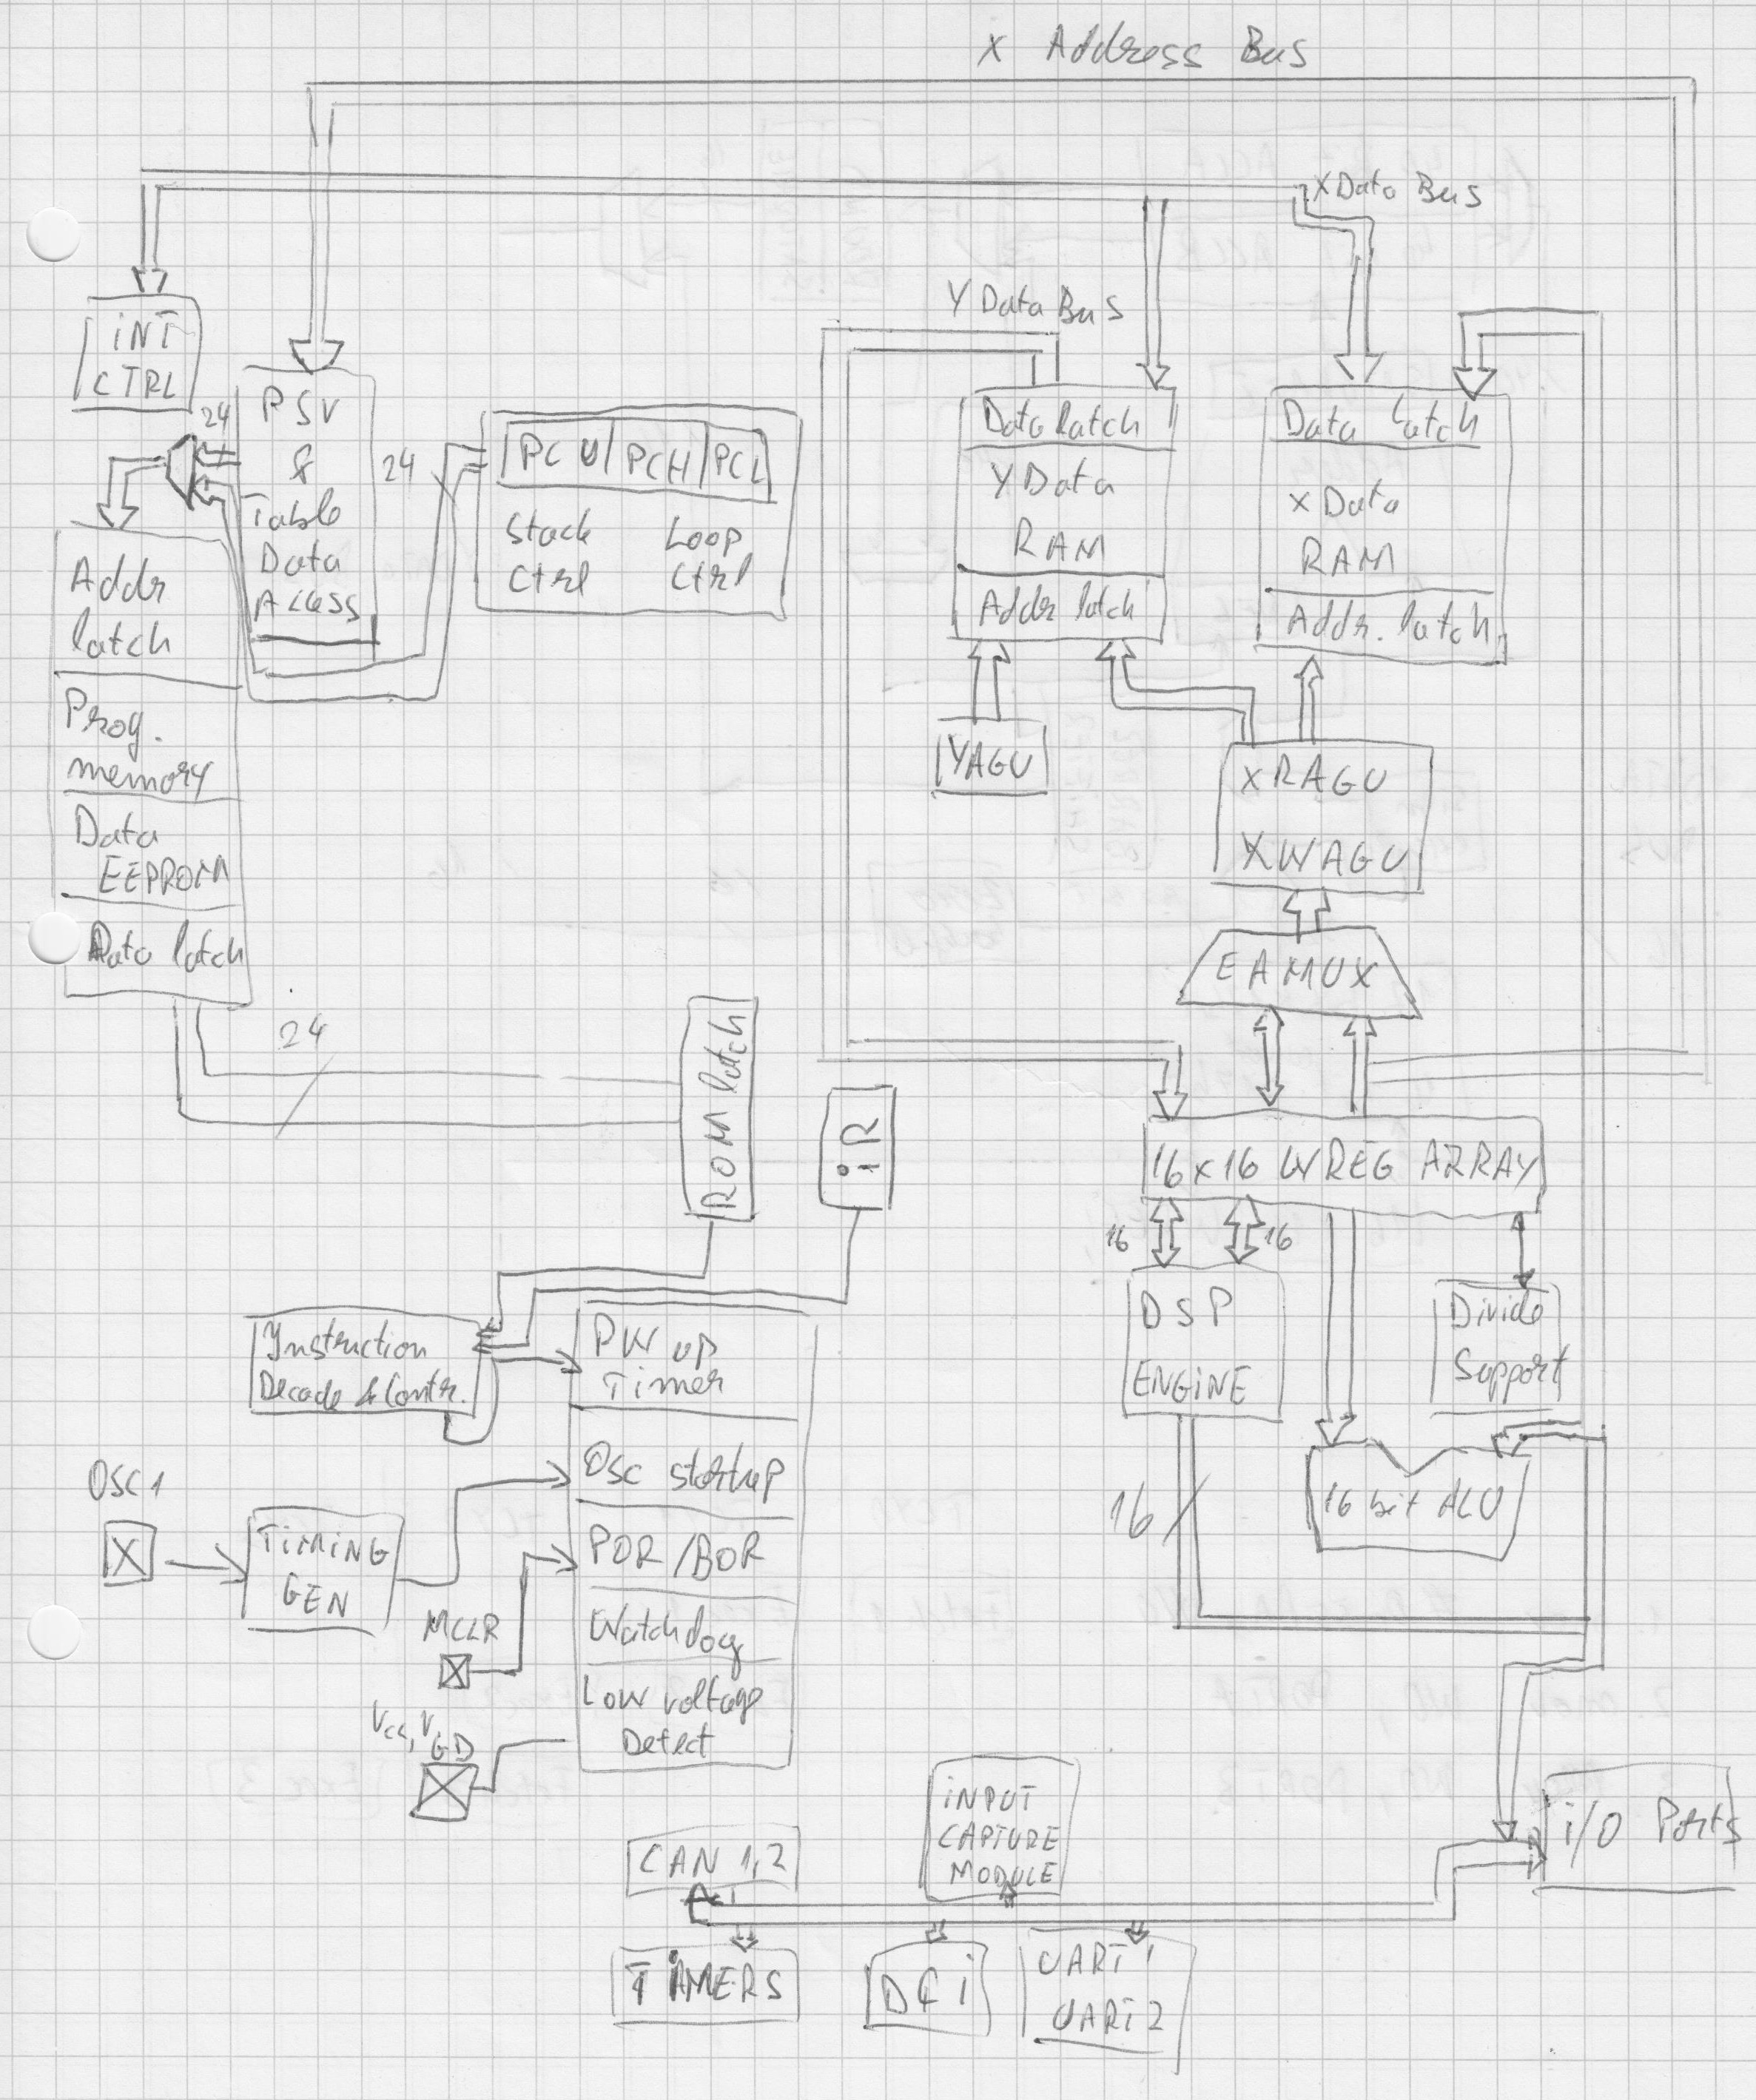
\includegraphics[scale=0.13]{figures/dsp_cpu.jpg}
    \caption{Processzor architektúra}
\end{figure}

\subsection{CPU regiszterek}

Fontosabb regiszterek:

\begin{itemize}
    \item W4, W5, W6, W7 - operandus regiszterek
    \item W8, W9, W10, W11 - címregiszterek (W8 és W9 - X memóriának, W10 és W11 - Y memóriának)
    \item W14 - frame pointer
    \item W15 - stack pointer
    \item CORCON - CPU viselkedését módosító flag-eket tartalmazó regiszter
    \item ACCA és ACCB - 40 bites akkumulátorok (3 darab 16 bites regiszterben vannak eltárolva)
\end{itemize}

\subsection{Aritmetikai és logikai egység}

Az ALU (Arithmetic Logic Unit) képes összeadást, kivonást, logikai műveleteket és egybites eltolást elvégezni. Az operandusokat a W regiszterekből vagy az adatmemóriából jönnek, az eredmény kerülhet ugyancsak a W regiszterbe vagy az adatmemóriába. 

\subsection{DSP motor}

A DSP motor viselkedését a CORCON regiszter bitjeit állítva tudjuk módosítani:

\begin{itemize}
    \item IF: egész vagy törtszámos szorzást végezzen
    \item US: előjeles vagy előjel nélküli számokkal dolgozzon
    \item SATA: legyen A regiszterre telítés vagy sem
    \item SATB: legyen a B regiszterre telítés vagy sem
\end{itemize}

\begin{figure}[H]
    \centering
    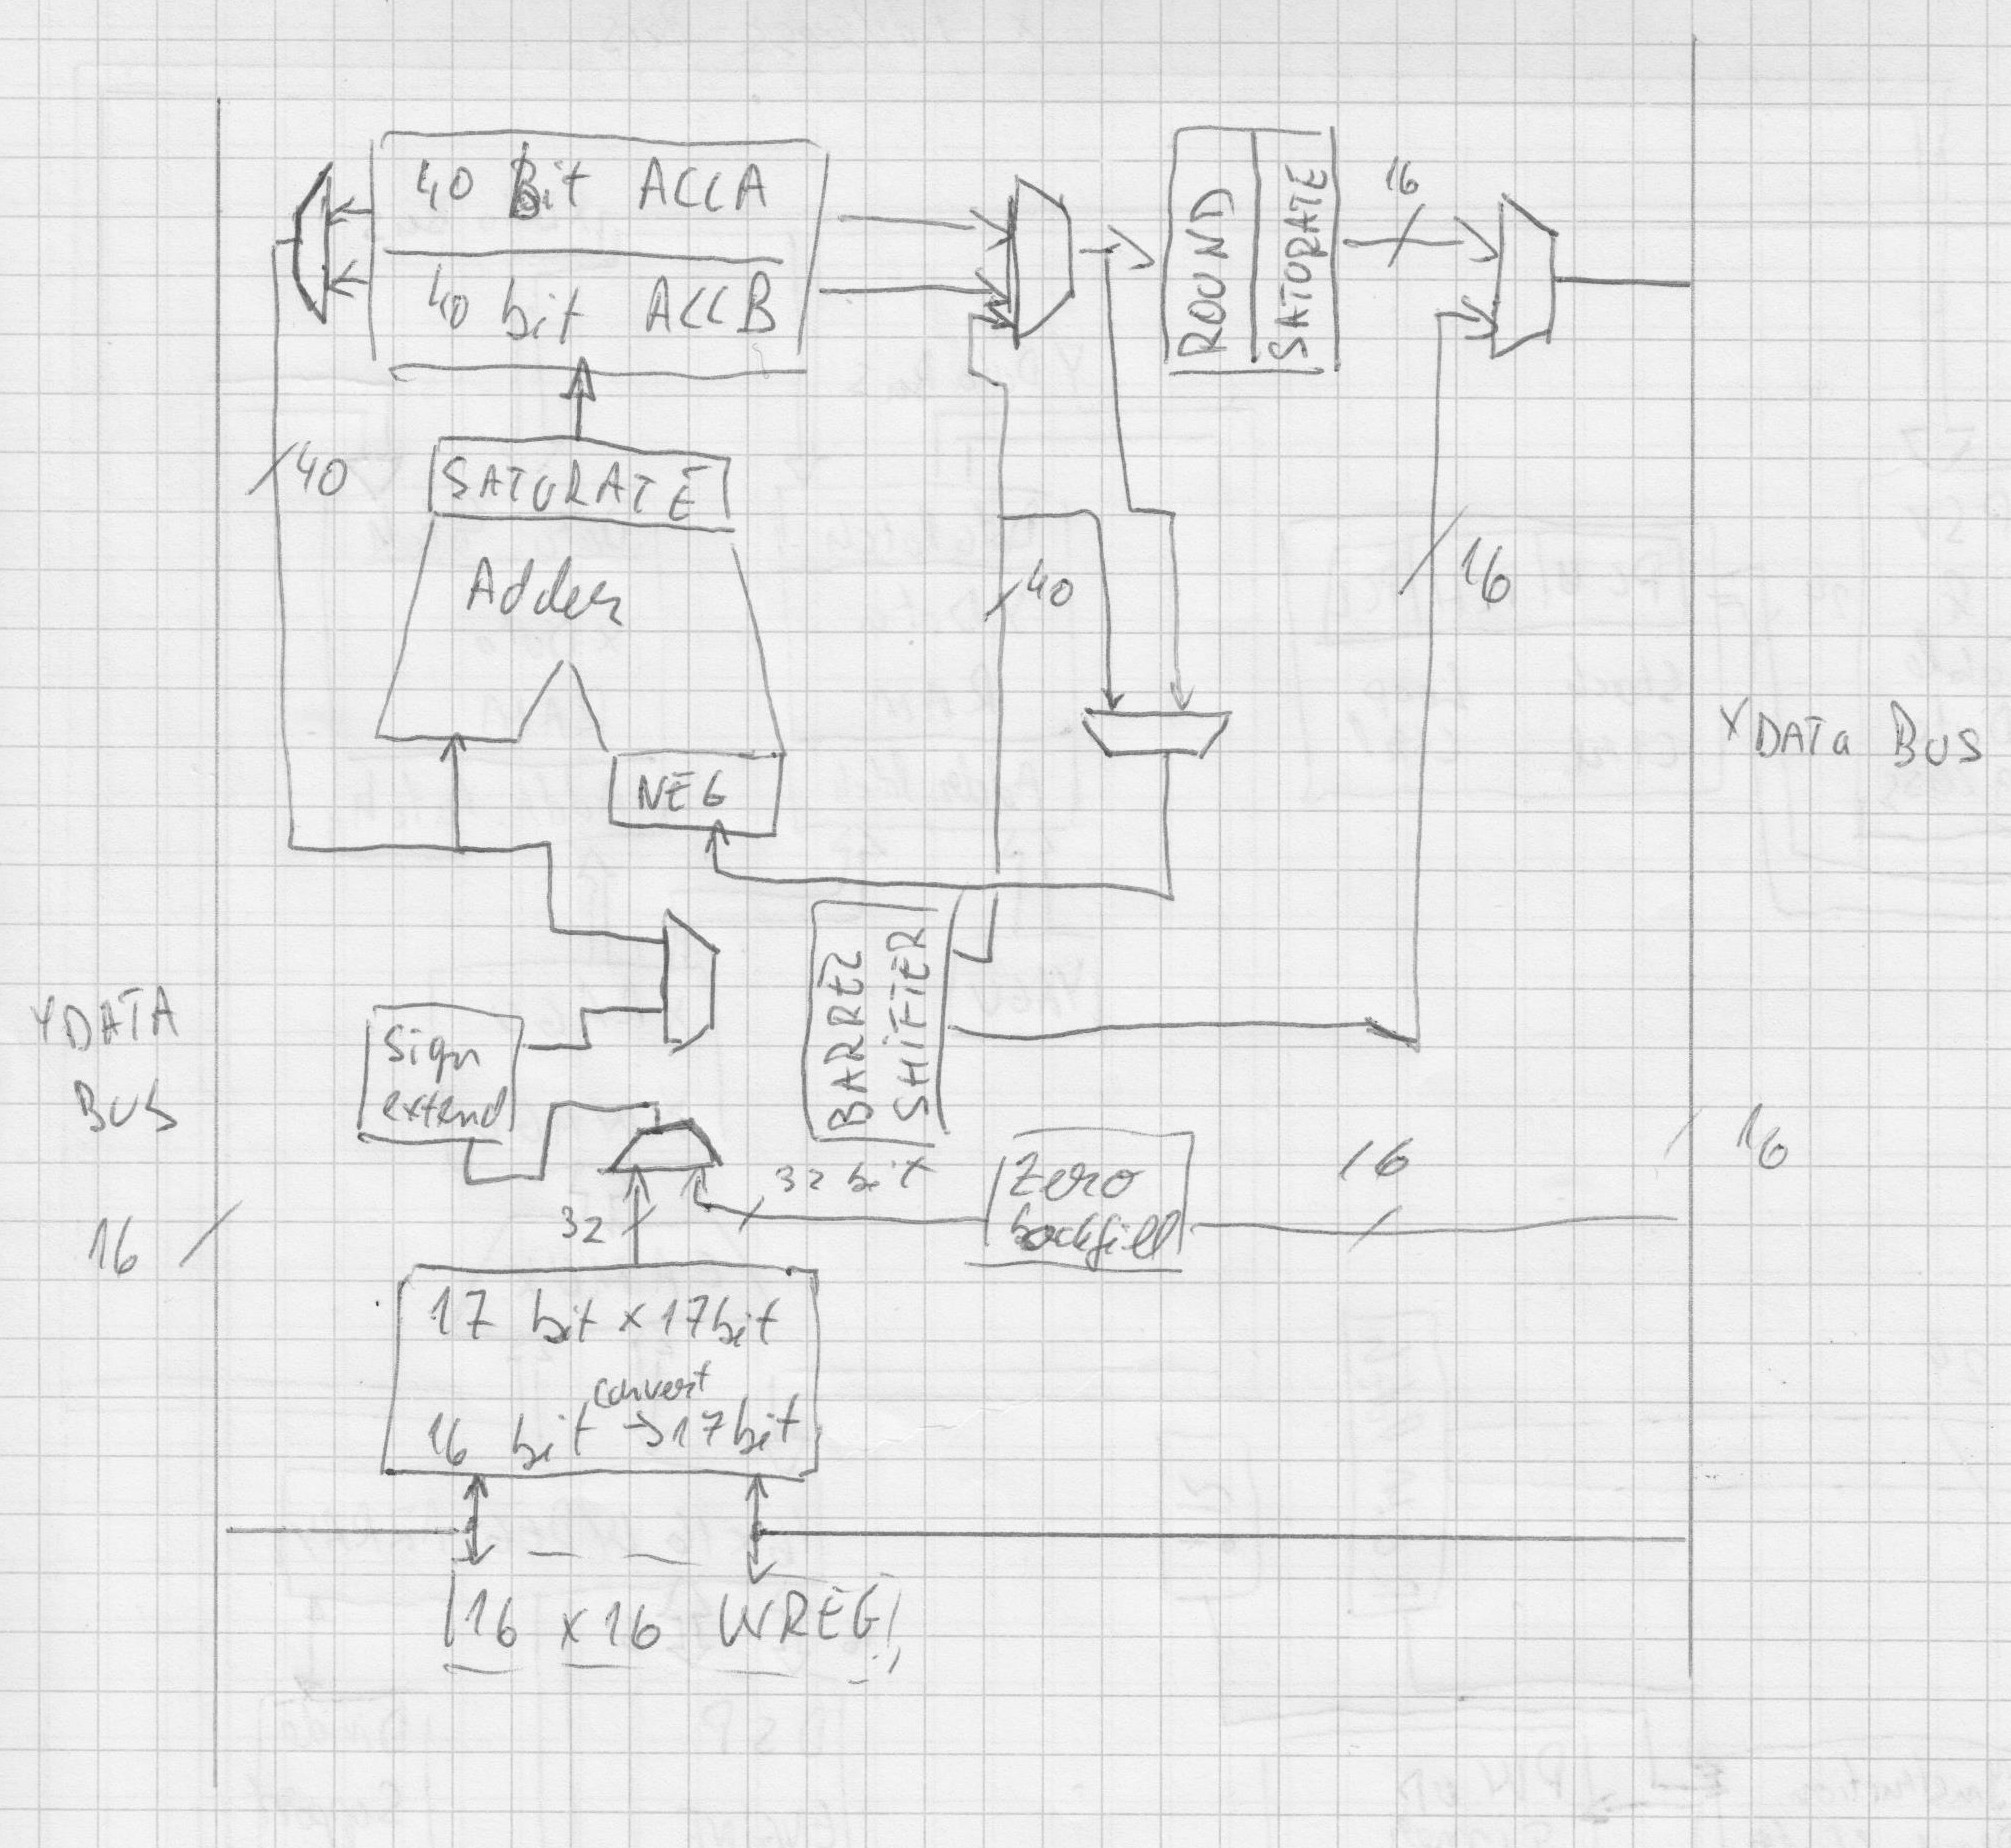
\includegraphics[scale=0.15]{figures/dsp_engine.jpg}
    \caption{DSP motor}
\end{figure}

\subsection{DSP utasítások}

\begin{itemize}
    \item mac: $a = a + b * c$ (multiply and accumulate)
    \item msc: $a = a - b * c$ (multiply and subtract)
    \item mpy: $a = b * c$ (multiply)
    \item mpy.n: $a = - b * c$ (multiply and negate)
    \item ed: $a = (b - c) ^ 2$ (euclidean distance)
    \item edac: $a = a + (b - c) ^ 2$ (euclidean distance and accumulate)
\end{itemize}

Példa: MAC W4*W5, A, [W8]+=2, W4, [W10]+=2, W5

Itt W4*W5 $\rightarrow$ A, [W8]+2 $\rightarrow$ W4, [W10]+2 $\rightarrow$ W5. Fontos, hogy a harmadik operandus (itt [W8]) X memóriát címző regiszter legyen és az ötödik operandus (itt [W10]) Y memóriát címző regiszter.

\subsection{Hardware osztó}

A dsPIC30F-nél az osztó blokk képes előjeles és előjel nélküli egész számok osztására. Az osztás hányadosa a W0 regiszterbe kerül és a maradék a W1-es regiszterbe. Műveletek:

\begin{itemize}
    \item DIVF: 16/16 előjeles törtszám osztás
    \item DIV.SD: 32/16 előjeles osztás
    \item DIV.UD: 32/16 előjel nélküli osztás
    \item DIV.UW: 16/16 előjel nélküli osztás
\end{itemize}

\subsection{Utasításciklusok}

A dsPIC-ek pipeline-ozott architektúrát használnak, amiből kifolyólag az egymás után követő utasítások nem kell megvárják amíg az azelőtti utasítás minden fázisa véghez ment (Fetch és Execute), hanem amíg az első utasítás az execute fázisban van, addig a második utasítás lehet a fetch fázisban. Ez gyorsításhoz és az erőforrások hatékonyabb kihasználásához vezet.

\begin{figure}[H]
    \centering
    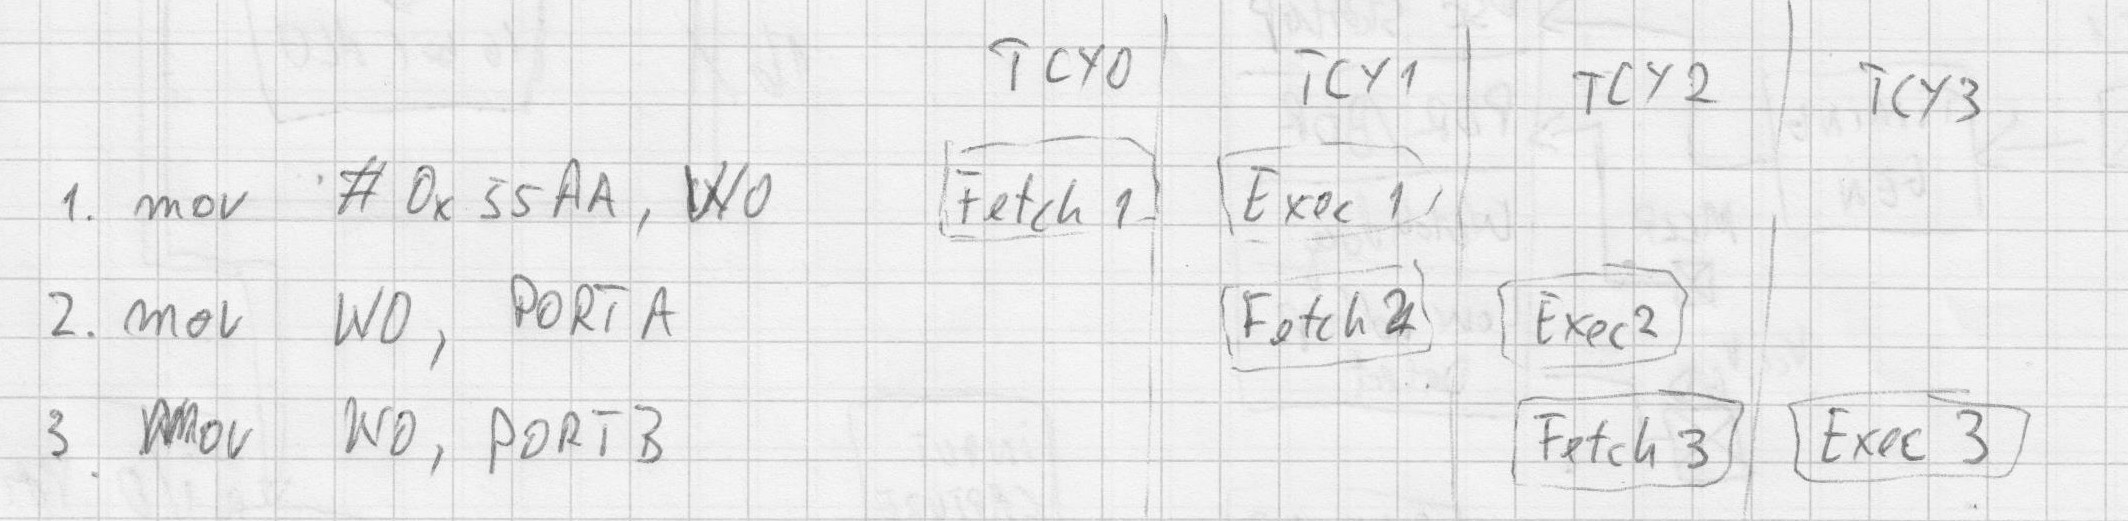
\includegraphics[scale=0.25]{figures/dsp_fetch_ex.jpg}
    \caption{Utasításciklusok}
\end{figure}
